\subsection{Ancient Tortoise}
    \subsubsection{Definición}
      \paragraph{El principal objetivo de este módulo es procesar y mostrar la información histórica de las variables almacenadas en las bases de datos de tipo MX. Ancient Tortoise tomará calculará y generará por medio de una regresión lineal una predicción, a lo más de un mes, de las variables ambientales y de contaminación de un estado o localidad en específico. \cite{30}}
      \paragraph{La información obtenida a demanda por el módulo Smart Owl será la fuente de información básica para generar los modelos de predicción necesarios. Éste no modificará la información existente en la base de datos, sólo obtendra la información y calculará los datos entre los rangos de fechas definidos por el usuario desde la interfaz generada en Friendly Dolphin.}
      \paragraph{El usuario final tendrá interacción con estas operaciones ya sea a través de un servicio REST o usando la interfaz web que proporciona Friendly Dolphin. El diagrama por bloques del módulo aisla el módulo de calculos matemáticos dejando sólo expuesto el servicio para consultas dado una localidad o estado de la Republica Mexicana considerando como límites una fecha inicial y final. El módulo proveerá la opción de exportar la información generada por éste en los formatos JSON y XML.}
      \newpage
      \begin{landscape}
      \subsubsection{Diagrama por bloques.}
        \paragraph{A continuación se mostrará el diagrama por bloques que define la estructura de Ancient Tortoise.}
        \begin{figure}[b!]
        \centering
        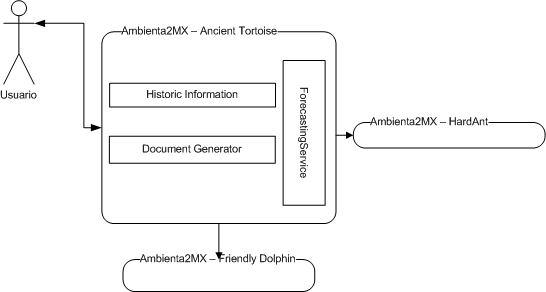
\includegraphics[width=22.5cm,height=12cm]{./images/DiagramaAncientTortoise.png}
        \caption{Diagrama General de Ancient Tortoise}
      \end{figure}
      \end{landscape}
      \newpage